\documentclass[a4paper, 12pt]{article}
\usepackage[T1]{fontenc}
\usepackage{lmodern}
\usepackage{color}
\usepackage{amsfonts}
\usepackage{epstopdf}
\usepackage{matlab}
%\documentclass{book}
\usepackage{blindtext}
\usepackage{hyperref}
\usepackage[brazil]{babel}
\usepackage{amssymb}
\usepackage[utf8]{inputenc}
\usepackage{amsmath}
\usepackage{indentfirst}
\usepackage{graphicx}
\usepackage{multicol,lipsum}
\usepackage[a4paper,
top=3cm, left=3cm, bottom=3cm, right=3cm]{geometry}
\usepackage{setspace}
\usepackage{multirow}
\usepackage{float}
\usepackage[dvipsnames]{xcolor}
\usepackage[table]{xcolor}
%\usepackage{pdflscape}
\usepackage[DIV=15]{typearea}
\usepackage[nottoc]{tocbibind}
\usepackage[sort,numbers]{natbib}
%\usepackage{cite}
\usepackage{matlab}

\usepackage[utf8]{inputenc}
\usepackage[T1]{fontenc}
\usepackage{lmodern}
\usepackage{graphicx}
\usepackage{color}
\usepackage{hyperref}
\usepackage{amsmath}
\usepackage{amsfonts}
\usepackage{epstopdf}
\usepackage[table]{xcolor}
\usepackage{matlab}


\documentclass[letterpaper]{article}
% bib pack %%%%%%%%%%%%%%%%%%%%%%%%%%%%%%%%%%%%%%%%%%%%%%%%%%%%%%%%%%%%%%%%%%%%%
\usepackage[utf8]{inputenc}
\usepackage{geometry}
    \geometry{left=3cm,right=2cm,top=2cm,bottom=2cm}
%
\usepackage[spanish]{babel}
%
\usepackage[fixlanguage]{babelbib}
    \bibliographystyle{babunsrt}
%
\usepackage{url}

\begin{document}
%\maketitle

\begin{titlepage}
	\begin{center}
		

\vspace{10pt}
%\begin{figure}[H][!ht]
%\centering
%
\includegraphics{puc-rio-logo.png}

%\end{figure}
\begin{figure}[!ht]
\centering

\includegraphics{images/puc-rio-logo.png}
\end{figure}
\huge{Dinâmica de Sistemas}
        \vspace{70pt}
        
		\textbf{ENG1730}
		\textbf{\large{\\ }}
		
		\vspace{30pt}
		\textbf{\small{\\Lista 01}}
		\vspace{75pt}
		
	\end{center}
	
	\begin{flushleft}
		\begin{tabbing}
			Aluno(a)\qquad\qquad\=\>Paloma Fernanda Loureiro Sette - 1621595\\
			
			Professor(a)\>João Carlos Virgolino Soares\\
	\end{tabbing}
		  
	\end{flushleft}
	\begin{center}
		%\vspace{\fill}
		\vspace{215pt}
		Rio de Janeiro, 07 de Setembro de 2022
	\end{center}
\end{titlepage}
%%%%%%%%%%%%%%%%%%%%%%%%%%%%%%%%%%%%%%%%%%%%%%%%%%%%%%%%%%%
\newpage
\tableofcontents
\thispagestyle{empty}

\newpage
\pagenumbering{arabic}

\newpage

%\newcommand{\listequationsname}{Lista de Equações}
%\newlistof{myequations}{equ}{\listequationsname}
%\newcommand{\myequations}[1]{%
%\addcontentsline{equ}{myequations}{\protect\numberline{\theequation}#1}\par}

%\listofmyequations
\newpage


\newpage

\listoffigures
\thispagestyle{empty}

\newpage
%%%%%%%%%%%%%%%%%%%%%%%%%%%%%%%%%%%%%%%%%%%%%%%%%%%%%%%%%
%%%%%%%%%%%%%%%%%%%%%%%%%%%%%%%%%%%%%%%%%%%%%%%%%%%

\newpage

\thispagestyle{empty}

\newpage

\section{Introdução}
Este relatório refere-se ao primeiro trabalho da disciplina de Dinâmica de Sistemas, ENG1730, de 2022.2. Trataremos de modelagem e simulações de sistemas mecânicos massa-mola, utilizando Simulink e MATLAB, de acordo com a programação do curso.

\section{Questão 01}
Consideremos o sistema massa-mola da figura seguinte, com massa \textbf{m} atrelada a três molas de constantes \textbf{k1}, \textbf{k2} e \textbf{k3}.

\begin{figure}[H]
\centering
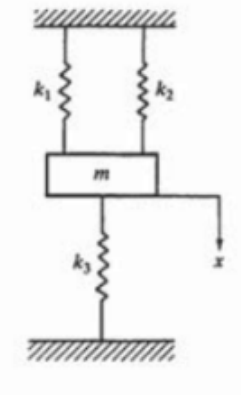
\includegraphics[scale = 0.7]{images/q01.png}
\label{filtro1}
\caption{Sistema massa-mola - questão 01}
\end{figure}

\subsection{Modelo matemático do sistema}
A princípio, podemos gerar o Diagrama de Corpo Livre do sistema, que já é de fácil visualização:

\begin{figure}[H]
\centering
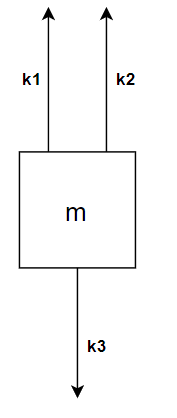
\includegraphics[scale = 0.7]{images/DCL_q01.png}
\label{filtro1}
\caption{Diagrama de Corpo Livre - questão 1.1}
\end{figure}

A partir do D.C.L. do sistema, representado na figura acima, podemos obter, analíticamente, o modelo matemático.\\

Temos que:

\begin{equation}
    F_1 = K_1x
\end{equation}
\begin{equation}
    F_2 = k_2x
\end{equation}
\begin{equation}
    F_3 = k_3x
\end{equation}


\begin{equation}
    \sum{\vec{F}} = \vec{k_1} + \vec{k_2} + \vec{k_3}
\end{equation}

E sabemos que $F = m\ddot{x}$, logo,

\begin{equation}
    m\ddot{x} = x(k_1+k_2+k_3)
\end{equation}\\

Então, o modelo matemático do sistema é o seguinte:

\begin{equation}
    \ddot{x} = \frac{x}{m}(k_1+k_2+k_3)
\end{equation}

Tomaremos este modelo por base para gerarmos as simulações posteriormente.

\subsection{Resposta Dinâmica}

Devemos, nesta etapa, encontrar a resposta dinâmica do sistema (posição do bloco em função do tempo) com o auxílio do Simulink, a partir do modelo matemático que geramos no tópico anterior.\\

No Simulink, modelamos a resposta do sistema como é exibido na figura abaixo:

\begin{figure}[H]
\centering
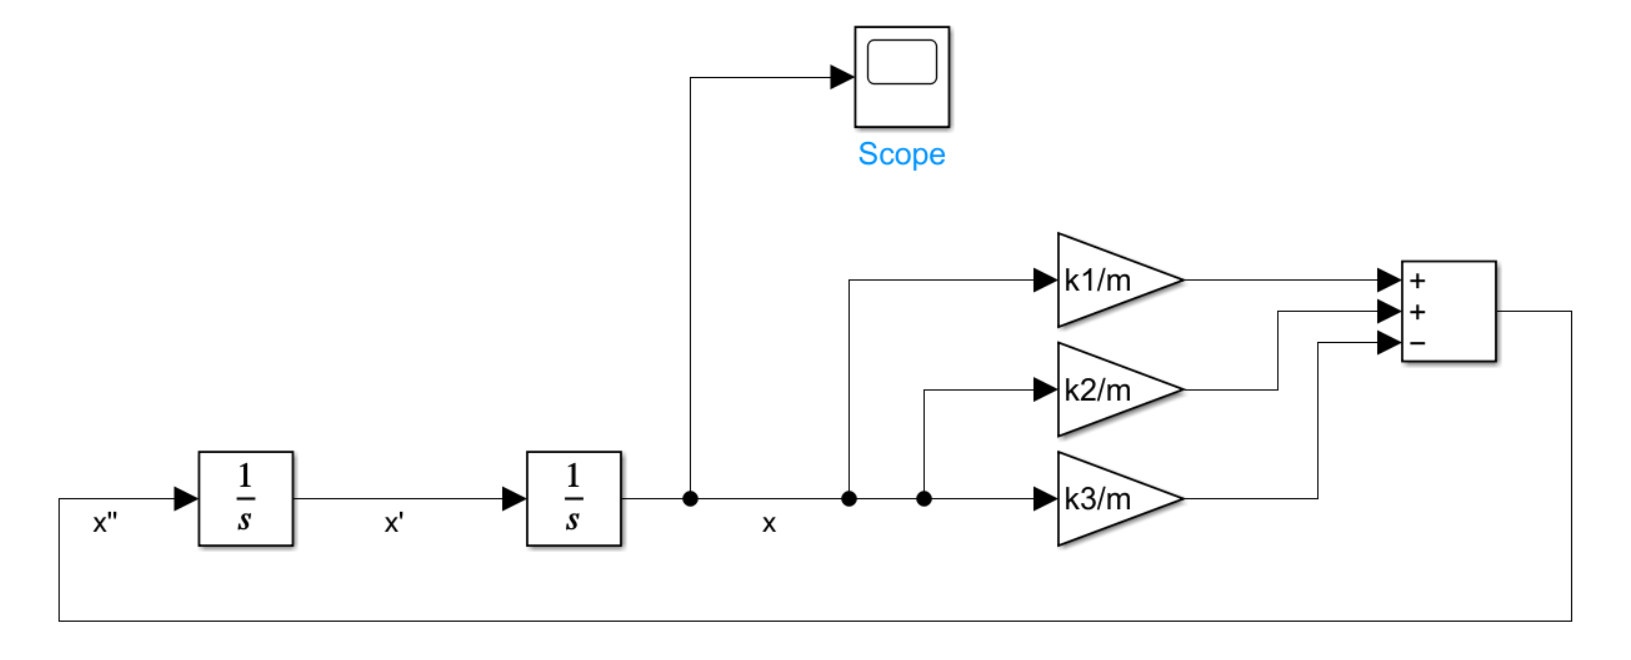
\includegraphics[scale = 0.35]{images/simulink01.png}
\label{filtro1}
\caption{Resposta Dinâmica com o Simulink}
\end{figure}

\subsection{Parâmetros do Sistema}

Foram inseridos os parâmetros no MATLAB, como é mostrado no código de MATLAB a seguir. Neste item, selecionamos os determinados valores de forma a exemplificar o funcionamento do sistema.

% This LaTeX was auto-generated from MATLAB code.
% To make changes, update the MATLAB code and export to LaTeX again.


\sloppy
\epstopdfsetup{outdir=./}
\graphicspath{ {./L01_Latex_images/} }


\begin{matlabcode}
%% Lista 01

close all
clear
clc

% Parametros do sistema massa-mola

x0 = 1; % m
m = 70; % kg
k1 = 50; % N/m
k2 = 50; % N/m
k3 = 40; % N/m
\end{matlabcode}

\subsection{Resposta Gráfica}

Neste item, é necessário que geremos os gráficos de posição/velocidade do bloco em função do tempo, usando os seguintes parâmetros iniciais no script criado anteriormente:\\


x inicial = 0.5m;\\
k1 = 50N/m;\\
k2 = 10N/m;\\
k3 = 150N/m e\\
m = 5kg\\

Então, no MATLAB, teremos o seguinte:
% This LaTeX was auto-generated from MATLAB code.
% To make changes, update the MATLAB code and export to LaTeX again.


\sloppy
\epstopdfsetup{outdir=./}
\graphicspath{ {./L01_Latex_images/} }


\begin{matlabcode}
%% Lista 01

close all
clear
clc

% Parametros do sistema massa-mola

x0 = 0.5; % m
m = 5; % kg
k1 = 50; % N/m
k2 = 10; % N/m
k3 = 150; % N/m
\end{matlabcode}

Portanto, a resposta gráfica que obtivemos para a posição e velocidade encontra-se nas figuras \ref{figura 5} e \ref{figura 6}. Para este item, inserimos o elemento \textit{scope}  também na conexão entre os integradores de $\ddot{x}$ e de $\dot{x}$. 

\begin{figure}[H]
\centering
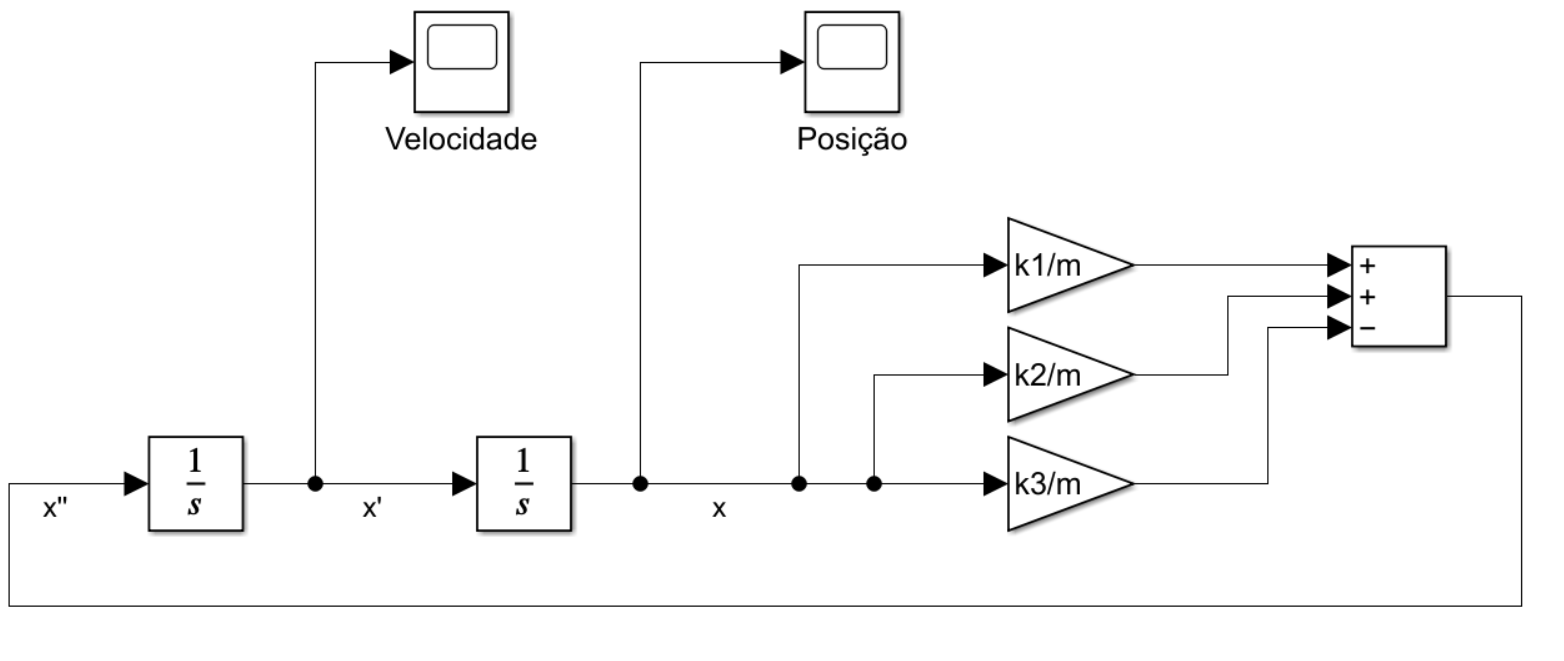
\includegraphics[scale = 0.35]{images/simulink02.png}
\label{filtro1}
\caption{Resposta dinâmica com adição de resposta gráfica para a velocidade}
\end{figure}

\begin{figure}[H]
\centering
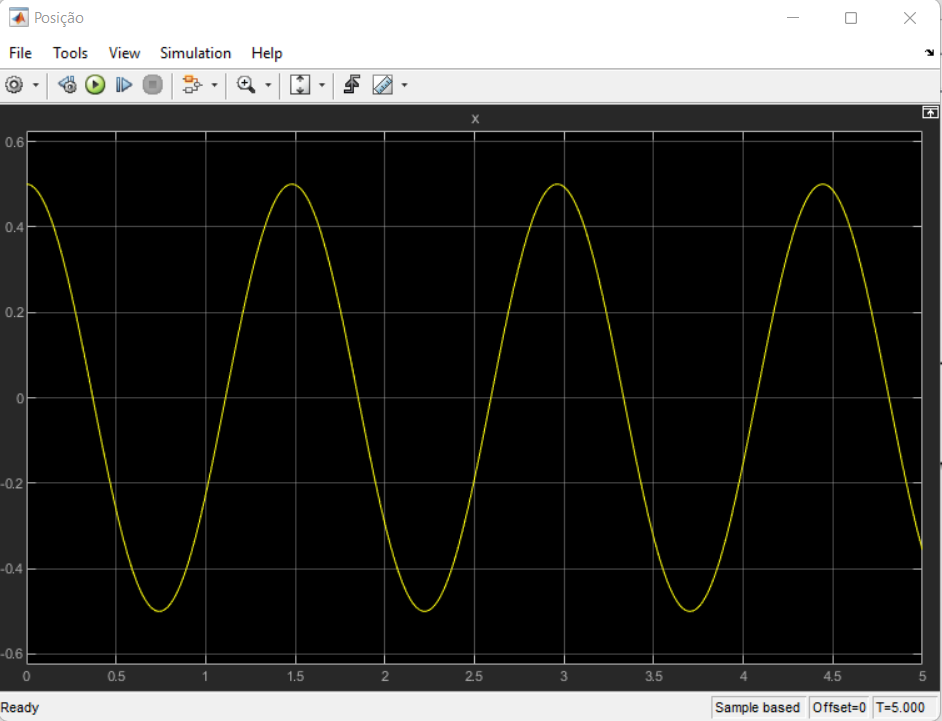
\includegraphics[scale = 0.5]{images/scope_posicao.png}
\label{filtro1}
\caption{Resposta gráfica para a posição}
\label{figura 5}
\end{figure}

\begin{figure}[H]
\centering
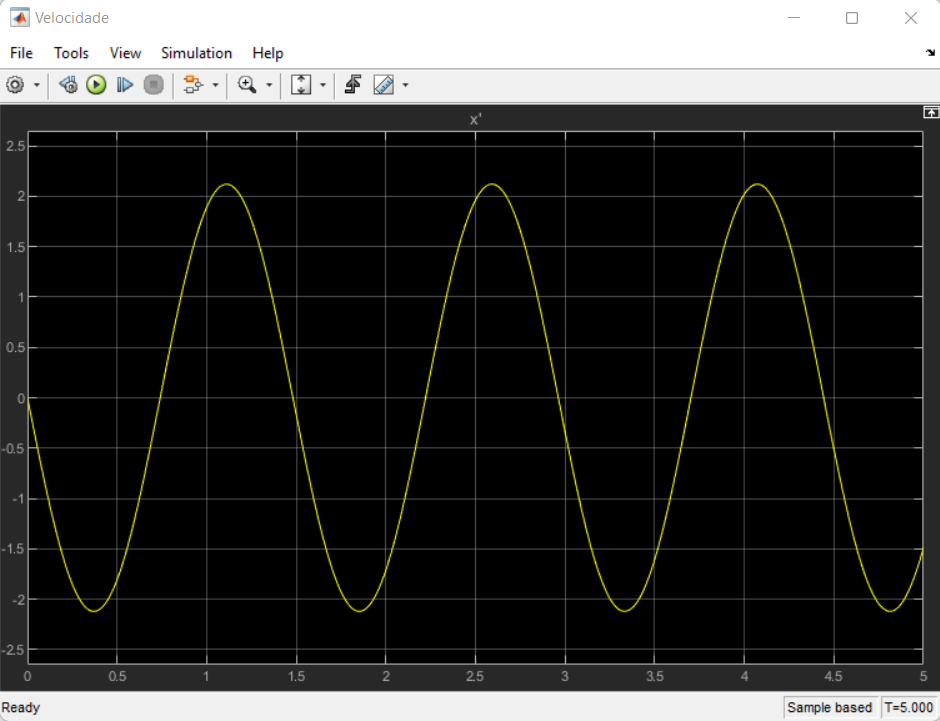
\includegraphics[scale = 0.5]{images/scope_velocidade.png}
\label{filtro1}
\caption{Resposta gráfica para a velocidade}
\label{figura 6}
\end{figure}


\subsection{Por que a posição da massa não vai a zero?}
Podemos notar, com base nas respostas gráficas, que a posição da massa nunca se anula. Conseguimos assimilar melhor esta situação quando comparamos com o caso em que houvesse um elemento amortecedor no sistema (se considerássemos o atrito com o ar, por exemplo). Isto é, com a amortecimento, teríamos a amplitude gráfica tendendo a zero com o passar do tempo, neste caso, com a velocidade sendo reduzida e a massa se tornando inerte.

Como não temos a consideração de qualquer amortecimento e sabemos que a mola armazena energia continuamente, essa energia nunca será dissipada. Desse modo, a energia mecânica total do sistema permanece constante ao longo de todo o movimento. Essa energia mecânica, por sua vez, é dada pela soma da energia cinética com a energia potencial elástica.

\subsection{Mudança de Parâmetros}

Neste item, devemos alterar os parâmetros no sistema para que a frequência de oscilação seja maior.
-Para este caso, podemos, por exemplo, multiplicar os parâmetros \textbf{k1}, \textbf{k2} e \textbf{k3} por 10, ficando da seguinte forma:

\sloppy
\epstopdfsetup{outdir=./}
\graphicspath{ {./L01_Latex_images/} }


\begin{matlabcode}
%% Lista 01

close all
clear
clc

% Parametros do sistema massa-mola

x0 = 0.5; % m
m = 5; % kg
k1 = 500; % N/m
k2 = 100; % N/m
k3 = 1500; % N/m
\end{matlabcode}


Assim, obtendo os gráficos exibidos nas figuras \ref{figura 7} e \ref{figura 8}.

\begin{figure}[H]
\centering
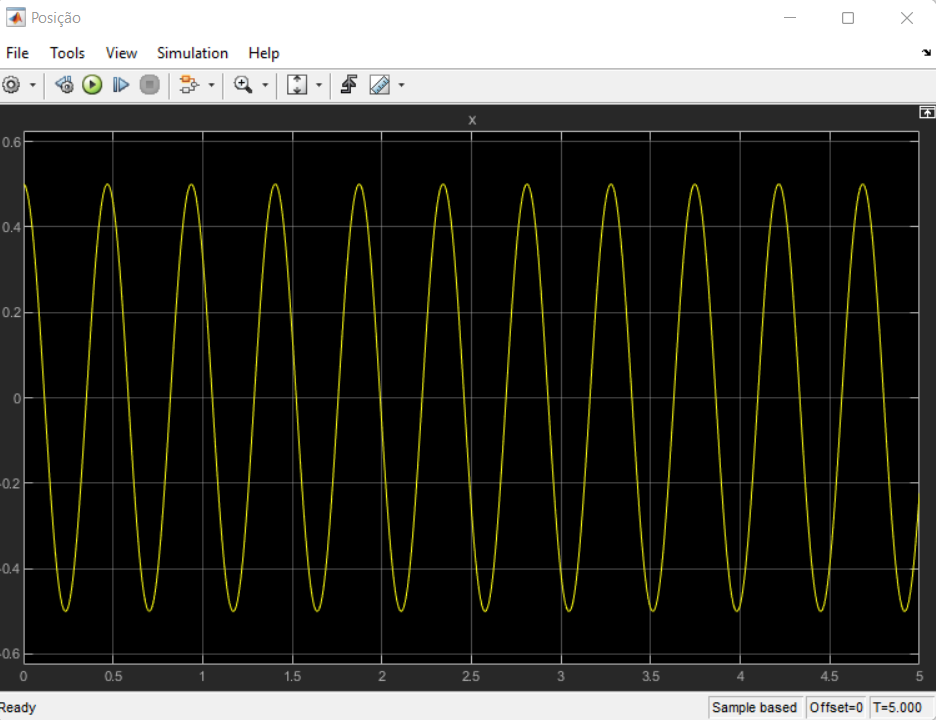
\includegraphics[scale = 0.5]{images/scope_posicaomaior.png}
\label{filtro1}
\caption{Resposta gráfica para a posição}
\label{figura 7}
\end{figure}

\begin{figure}[H]
\centering
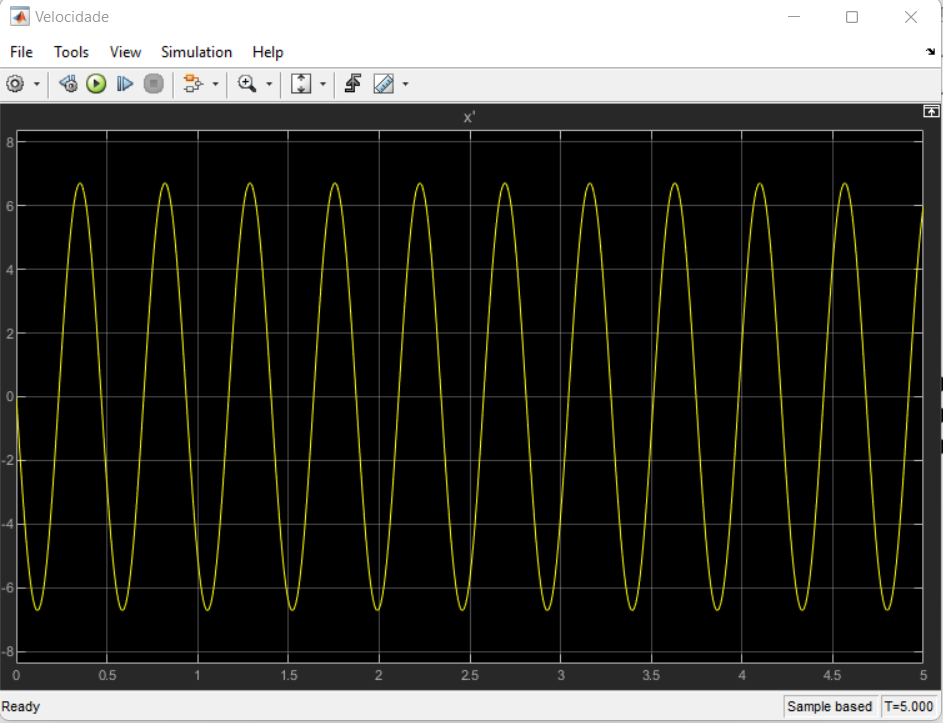
\includegraphics[scale = 0.5]{images/scope_velocidademaior.png}
\label{filtro1}
\caption{Resposta gráfica para a velocidade}
\label{figura 8}
\end{figure}


Neste caso, estamos aumentando muito a rigidez das molas e sabemos que os parâmetros de modelagem influem consideravelmente uns sobre os outros.
Quando a massa é retirada da posição de equilíbrio, a força elástica exercida pela mola faz com que o corpo passe a oscilar em torno dessa posição. 



Isto é, de acordo com as leis do Movimento Harmônico Simples, a frequência é diretamente proporcional à constante elástica da mola, ou seja, quanto mais rígida for esta mola, mais rápido será o movimento oscilatório do sistema.


\section{Questão 02}
A figura a seguir mostra um sistema com três molas com constantes \textbf{k1}, \textbf{k2} e \textbf{k3}. Devemos obter a mola equivalente do sistema.

\begin{figure}[H]
\centering
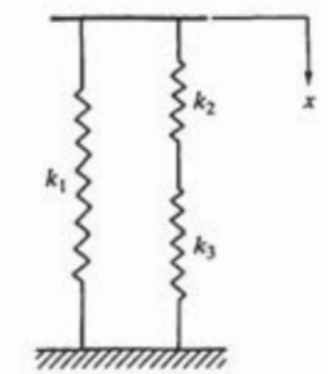
\includegraphics[scale = 0.7]{images/q02.png}
\label{filtro1}
\caption{Sistema mola - questão 02}
\end{figure}

Para esta questão, primeiramente, redesenhamos o sistema, de forma a evidenciar a posição que diz respeito à "y", como na figura \ref{figura 10}.

\begin{figure}[H]
\centering
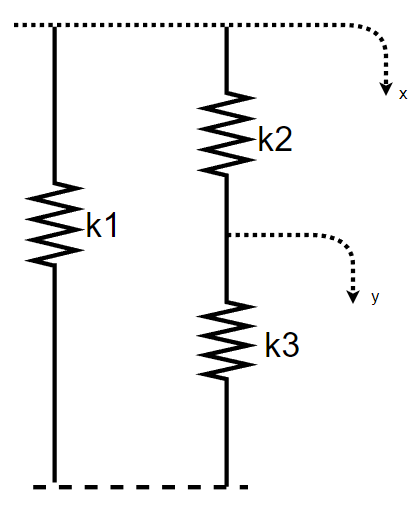
\includegraphics[scale = 0.45]{images/sistema_q02.png}
\label{filtro1}
\caption{Sistema mola redesenhado - questão 02}
\label{figura 10}
\end{figure}

Então, podemos considerar a princípio o sistema de molas em série, para obtermos um valor $k_{eq1}$ e, posteriormente, $k_{eq}$ do sistema como um todo, considerando as molas em paralelo.

\paragraph{Para as molas em série}:\\

\begin{equation}
    F_1 = k_3y
\end{equation}


\begin{equation}
    F_1 = k_2(x-y) \longrightarrow F_1 = k_2(x - \frac{F_1}{k_3})
\end{equation}

\begin{equation}
    k_2x = F_1 + \frac{k_2}{k_3}F_1
\end{equation}

\begin{equation}
    x = (\frac{k_3 + k_2}{k_3k_2})
\end{equation}

Agora, podemos considerar o sistema representado na figura \ref{figura 11} e teremos:

\begin{equation}
    F = k_{eq1}x
\end{equation}

sendo 

\begin{equation}
k_{eq1} = \frac{k_3 + k_2}{k_3k_2}    
\end{equation}

\paragraph{Para as molas em paralelo}:\\

Agora, com o sistema em paralelo, como mostrado na figura \ref{figura 11}, fica mais simples de obtermos a mola equivalente do sistema.

\begin{figure}[H]
\centering
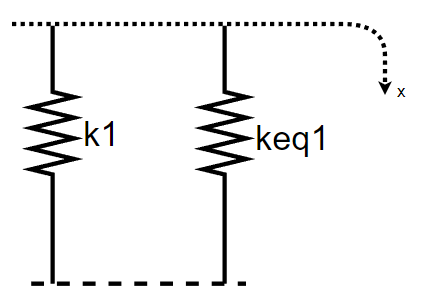
\includegraphics[scale = 0.5]{images/k_keq1.png}
\label{filtro1}
\caption{Sistema mola reduzido - questão 02}
\label{figura 11}
\end{figure}

\begin{equation}
    F = F_1 + F_2
\end{equation}


\begin{equation}
    F = k_1x + k_{eq1}x
\end{equation}


\begin{equation}
    F = (k_1 + k_{eq1})x
\end{equation}

Sabemos que


\begin{equation}
    F = k_{eq}x
\end{equation}

Então, teremos:


\begin{equation}
    k_{eq} = k_1 + k_{eq1} 
\end{equation}

Logo,


\begin{equation}
    k_{eq} = k_1 + \frac{k_3+k_2}{k_3k_2}
\end{equation}
\section{Questão 03}
Devemos implementar uma função no MATLAB que receba um vetor \textbf{x}, calculando também o valor de $y = 2 cos(3x)$ e, em seguida, plotar o gráfico $(x,y)$. Devemos testar com um vetor de, no mínimo, 101 elementos com valores crescentes de 0 até 10.
Implementaremos a operação $y = 2 cos(3x)$ no Simulink de forma a obter os mesmos resultados do MATLAB.

\begin{matlabcode}
%% Lista 01 - questão 03
%% Paloma Sette - 1621595

%definição da função

function y = func(x) 
%y é a variavel de saída da função
%func é o nome da função, será o vetor de valores de 0 a 10 passados
% na função 2cos(3x).

y = [];

for i = 1:length(x)
    if x(i) >= 0 & x(i) <= 10 
        y = [y 2*cos(3*x(i))];
    end
end

end

\end{matlabcode}

Em seguida, o código utilizado para fazer o uso da função.

\begin{matlabcode}
%% Lista 01 - questão 03
%% Paloma Sette - 1621595

close all
clear
clc

x = randn(1, 115) %vetor que gera numeros aleatorios

func(x)

figure
plot(x)
xlim([1 20])
ylim([-5 5])
grid on

\end{matlabcode}

Neste exemplo, foi gerado o seguinte gráfico:

\begin{figure}[H]
\centering
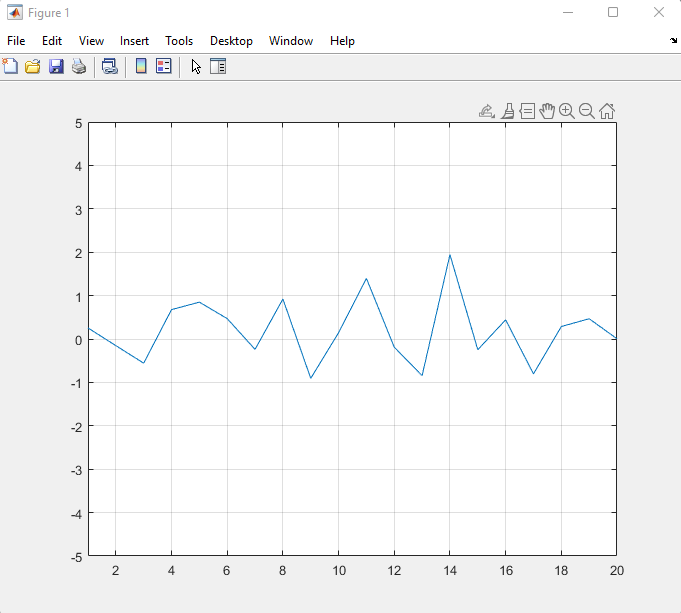
\includegraphics[scale = 0.65]{images/graph_q3.png}
\caption{Gráfico de exemplo - questão 03}
\end{figure}

No entanto, houve certa dificuldade para a geração da resposta com o Simulink, para fins de comparação neste item.

\newpage
% REFERENCIAS %%%%%%%%%%%%%%%%%%%%%%%%%%%%%%%%%%%%%%%%%%%%%%%%%%%%%%%%%%%%%%
    \nocite{*}
    \bibliography{src/bibliography}
    
\end{document}
\section{Referências Bibliográficas}



\end{document}